\chapter{Red recíproca y difracción de rayos X} \label{Ch:02}

El objetivo es estudiar cómo se utiliza la difracción de ondas por el cristal para determinar el tamaño de la celda, la posición de los átomos y la distribución de electrones dentro de la celda. Las radiaciones con longitud de onda $\lambda$ del orden la constante de red $a$   (algunos $ A$), {\it ven} la estructura atómica del cristal de modo que cada átomo en el cristal es un (re)emisor independiente. La onda difractada depende de todas las posiciones atómicas pues se trata de una \textit{interferencia interna} que es constructiva para ciertas direcciones de salida. A partir de la observación experimental de las \textit{direcciones de máximo} se obtiene importante información de la estructura del cristal. La radiación más utilizada son los rayos {\it x} (con $\lambda \sim a$) algunas de cuyas limitaciones son la dificultad de detectar elementos ligeros como el H, así como diferenciar entre átomos de número atómico próximo. Los electrones, por su menor penetración (interaccionan fuertemente), se utilizan para sondear superficies o capas delgadas. Los neutrones son utilizados para localizar el H en sólidos y sistemas biológicas y el estudio de estructuras magnéticas (gracias al espín).

\section{Red recíproca}

La \textit{red recíproca} es una red asociada a la red directa o real y que desempeña un papel fundamental en la teoría de la difracción, el estudio de las funciones de onda electrónicas cristalinas, etc.  Conjuto de $\kn$ que hacen que $e^{i\kn \cdot \rn}$ sea periódica en $\Rn$. 

\textbf{Concepto}. Considérese un conjunto de puntos que consituyen una red de Bravais, es decir, invariantes en cojunto por traslaciones en \textit{vectores de red}, $\Rn = u_1 \an_1 + u_2 \an_2 + u_3 \an_3$. Una red es una estrucutra \textit{multiperiódica} porque tiene periodicidades espaciales distintas según las direcciones. Una manera de establecerlas cuantitativamente es preguntarse cuáles son las ondas periódicas en la red; es decir, que vectores de onda $\kn$ satisfacen:

\begin{equation}
    e^{i\kn \cdot (\rn + \Rn)} = e^{i \kn \cdot \rn} \Longleftrightarrow  e^{i \kn \cdot \Rn} = 1 \Longleftrightarrow \kn \cdot \Rn = 2\pi \times \text{entero} \label{Ec:02-01-01}
\end{equation}
La condición \ref{Ec:02-01-01} exige que $\kn$ sea de la forma 

\begin{equation}
    \kn = v_1 \bn_1 + v_2 \bn_2 + v_3 \bn_3 \label{Ec:02-01-02}
\end{equation}
con los $v_i$ enteros y los $\bn$ cumpliendo que
\begin{equation}
    \bn_i \cdot \an_j = 2 \pi \delta_{ij}  \quad \text{con} \ \delta_{ij} = \left\lbrace \begin{array}{l}
        1 \ \text{si} \ i = j \\
        0 \ \text{si} \ i \neq j
    \end{array} \right. \label{Ec:02-01-03}
\end{equation}
Es posible obtener una expresión para los $\bn_i$ a partir de unos vectores base primitivos $\an_i$ de partidad, pues \ref{Ec:02-01-03} lo verifican los vectores dados por

\begin{equation}
    \begin{split}    
    \bn_1 & = 2 \pi \frac{\an_2 \times \an_3}{\an_1 (\an_2 \times \an_3)} \\
    \bn_2 & = 2 \pi \frac{\an_3 \times \an_1}{\an_1 (\an_2 \times \an_3)}  \\
    \bn_3 & = 2 \pi \frac{\an_1 \times \an_2}{\an_1 (\an_2 \times \an_3)}
    \end{split}\label{Ec:02-01-04}
\end{equation}
Los vectores de la forma \ref{Ec:02-01-04}, que se denotarán de ahora en adelante por $\Gn$ forman una red llamada \textit{red recíproca}. Destacamos que la celda de Wigner-Seitz de la red recíproca se denomina \textit{primera zona de Brillouin} (PZB). 

La obtención de redes recíprocas asociadas a redes directas exige trabajar con vectores base primitivos pues sólo entonces la ecuación \ref{Ec:02-01-04} es válida. Como ejemplo, considérense las tres redes del sistema cúbico. Denotando por $\hni, \hnj, \hnk$ los versores de las tres aristas del cubo convencional de arsita $a$, unos vectores base primitivos son:

\begin{equation*}
    \begin{array}{llll}
    sc) \quad &  \quad \an_1 = a \hni & \quad \an_2 = a \hnj & \quad \an_3 = a \hnk \\
    bcc)  \quad & \quad \an_1 = \frac{a}{2} (-\hni+\hnj+\hnk) & \quad \an_2 = \frac{a}{2} (\hni-\hnj+\hnk)  & \quad \an_3 = \frac{a}{2} (\hni+\hnj-\hnk)  \\
    fcc) \quad & \quad \an_1 = \frac{a}{2} (\hnj + \hnk) & \quad \an_2 = \frac{a}{2} (\hni + \hnk) & \quad \an_3 = \frac{a}{2} (\hni + \hnj) \\
    \end{array}
\end{equation*}
Aplicando ahora las relaciones \ref{Ec:02-01-04} a los vectores base anteriores es fácil deducir que la red recíproca de la \textit{sc} es otra \textit{sc} de \textit{constante de red} $2\pi/a$; la red recíproca de la \textit{bcc} es una red \textit{fcc} con \textit{constante de red} $4\pi/a$; la de la \textit{fcc} es una \textit{bcc} con \textit{constante de red} $4 \pi/a$. 

\begin{figure}[h!] \centering
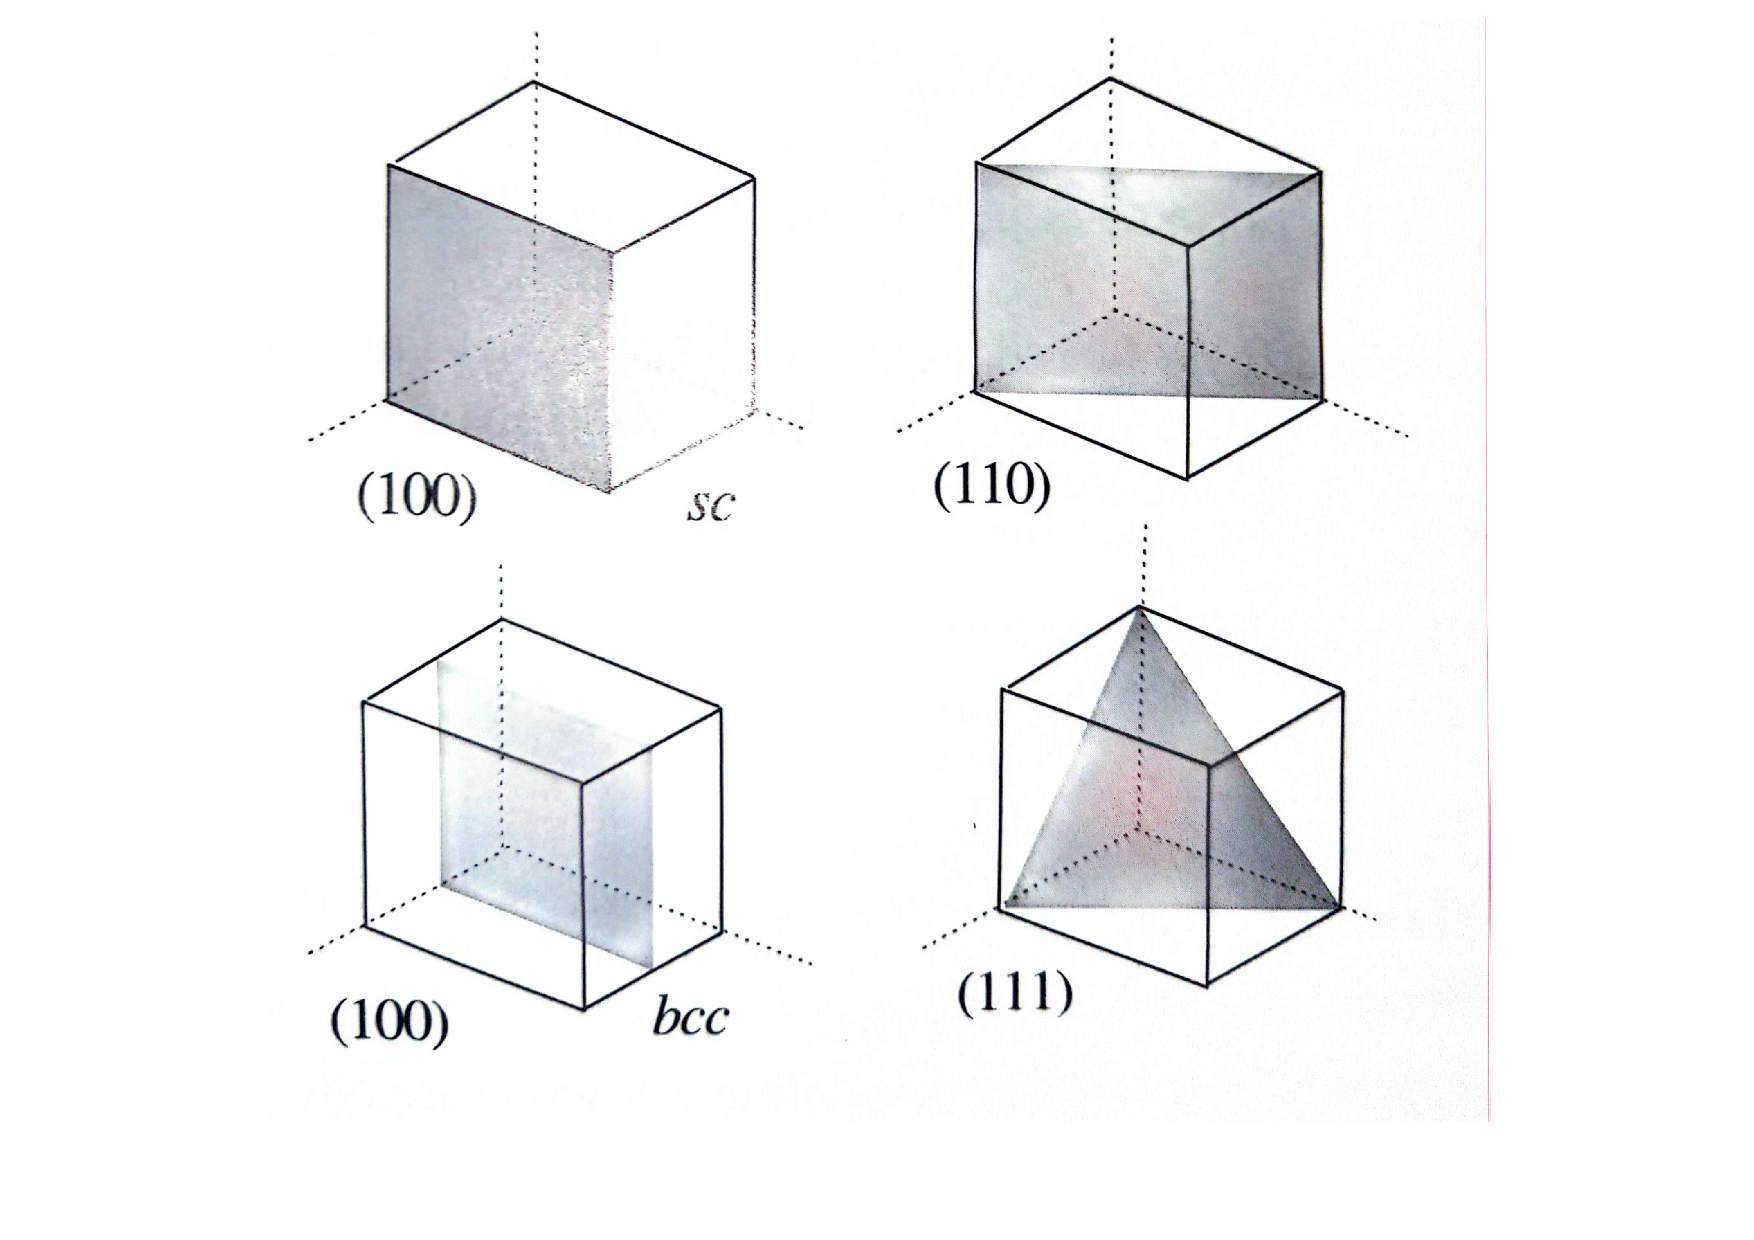
\includegraphics[scale=0.40]{Cuerpo/Ch_02/Fotos_libro 1.pdf}
\caption{Algunos planos reticulares para las redes cúbica simple (\textit{sc}) y centrada en el cuerpo (\textit{bcc}) y sus índices de Miller.}
\label{Fig:02-01}
\end{figure}

\begin{definition}[\textbf{Sistemas de planos reticulares: \textit{índices de Miller}}]. Por una familia o sistema de planos reticulares se entiende el cojunto de planos paralelos, equiespaciados, cada uno con el mismo número de puntos de red por unidad de área, que en conjuto contienen a todos los puntos de la red. A cada familia de planos se la hace corresponder tres índices como sigue: se toma cualquiera de los planos que no pase por el origen de coordenadas y se hallan los recíprocos de sus intersecciones sobre los ejes en unidades de las constantes de red $a,b,c$. La terna de números primos entre sí que están en la misma relación se denomina \textit{índices de Miller (hkl)}. En el caso del sistema cúbico (ver figura \ref{Fig:02-01}) los índices se entienden referidos a los ejes convencionales.    
\end{definition}


\textbf{Propiedades de la red recíproca}. Un resultado  geométrico interesante es el siguiente: para cualquier familia de \textit{índices de Miller (hkl)} separados por una distancia \textit{d}, el vector de la red recíproca $\Gn_0$ de componentes (\textit{hkl}) es perpendicular al sistema de planos y verifica que

\begin{equation}
|\Gn_0| = \frac{2\pi}{d} \label{Ec:02-01-05}
\end{equation}
Inversamente, para cualquier vector de la red recíproca $\Gn$ existe una familia de planos reticulares separados $d$, perpendiculares a $\Gn$ y tal que el vector de la red recíproca más corto paralelo a $\Gn$ verifica $|\Gn_0|=2\pi/d$. Una aplicación de este resultado es que el cálculo de la interdistancia $d$ entre planos adyacentes de una familia de planos se convierte en el cálculo de vectores de una red recíproca. Por ejemplo, en un \textit{sistema cúbico simple} sabemos que 

\begin{equation*}
    \bn_1 = \frac{2\pi}{a} \hni \quad \bn_2 = \frac{2\pi}{a} \hnj \quad \bn_3 = \frac{2\pi}{a} \hnk
\end{equation*}
son vectores primitivos de la red recíproca, por lo que $\Gn=h\bn_1+k\bn_2+l\bn_3$, siendo $h,k,l$ primos entre sí (esto es, no tienen un mínimo comúm multiplo). Entonces $G_0=\frac{2\pi}{a} \sqrt{h^2 + k^2 + l^2} \Rightarrow d = a/ \sqrt{h^2 + k^2 + l^2}$. 

Esto a su vez permite determinar de forma sencilla densidades planares: la densidad de puntos (puntos por unidad de área) $\sigma$ de un plano está relacionada con la densidad de la red $\rho$ por $\sigma/d = \rho$, y de aquí se puede determinar $\sigma$ a partir de $\rho$ y $d$. Otra propiedad útil de la red recíproca es que está relacionada con las magnitudes periódicas de la red. Un ejemplo puede ser la concentración electrónica $n(\rn)$.

\section{Difracción}

Sea una onda plana $e^{\kn \cdot \rn}$ incidente sobre un cristal. Vamos estudiar la amplitud de la onda dispersada en la dirección $\kn'$ (ver figura \ref{Fig:02-02}) suponiendo \textit{dispersión elástica} $(|\kn|=|\kn|')$

\begin{equation}
    A_{\text{salida}} \propto \sum_{m,n} f_{mn} e^{i \Delta \phi_{mn}}
\end{equation}
siendo $\Delta \phi_{mn} = (\kn - \kn') \cdot \dn_{mn}$ la diferencia de fase entre la onda reemitida por un centro dispersor ($m$) y otro ($n$) a $\dn_{mn}$ del primero. La suma ($m,n$) a todos los centros dispersores puede hacerse sumando a todas las celdas en \textit{posiciones de red} $\Rn_n$ y a todos los átomos de la base en posiciones $\rn_j$ dentro de cada celda. 

\begin{figure}[h!] \centering
    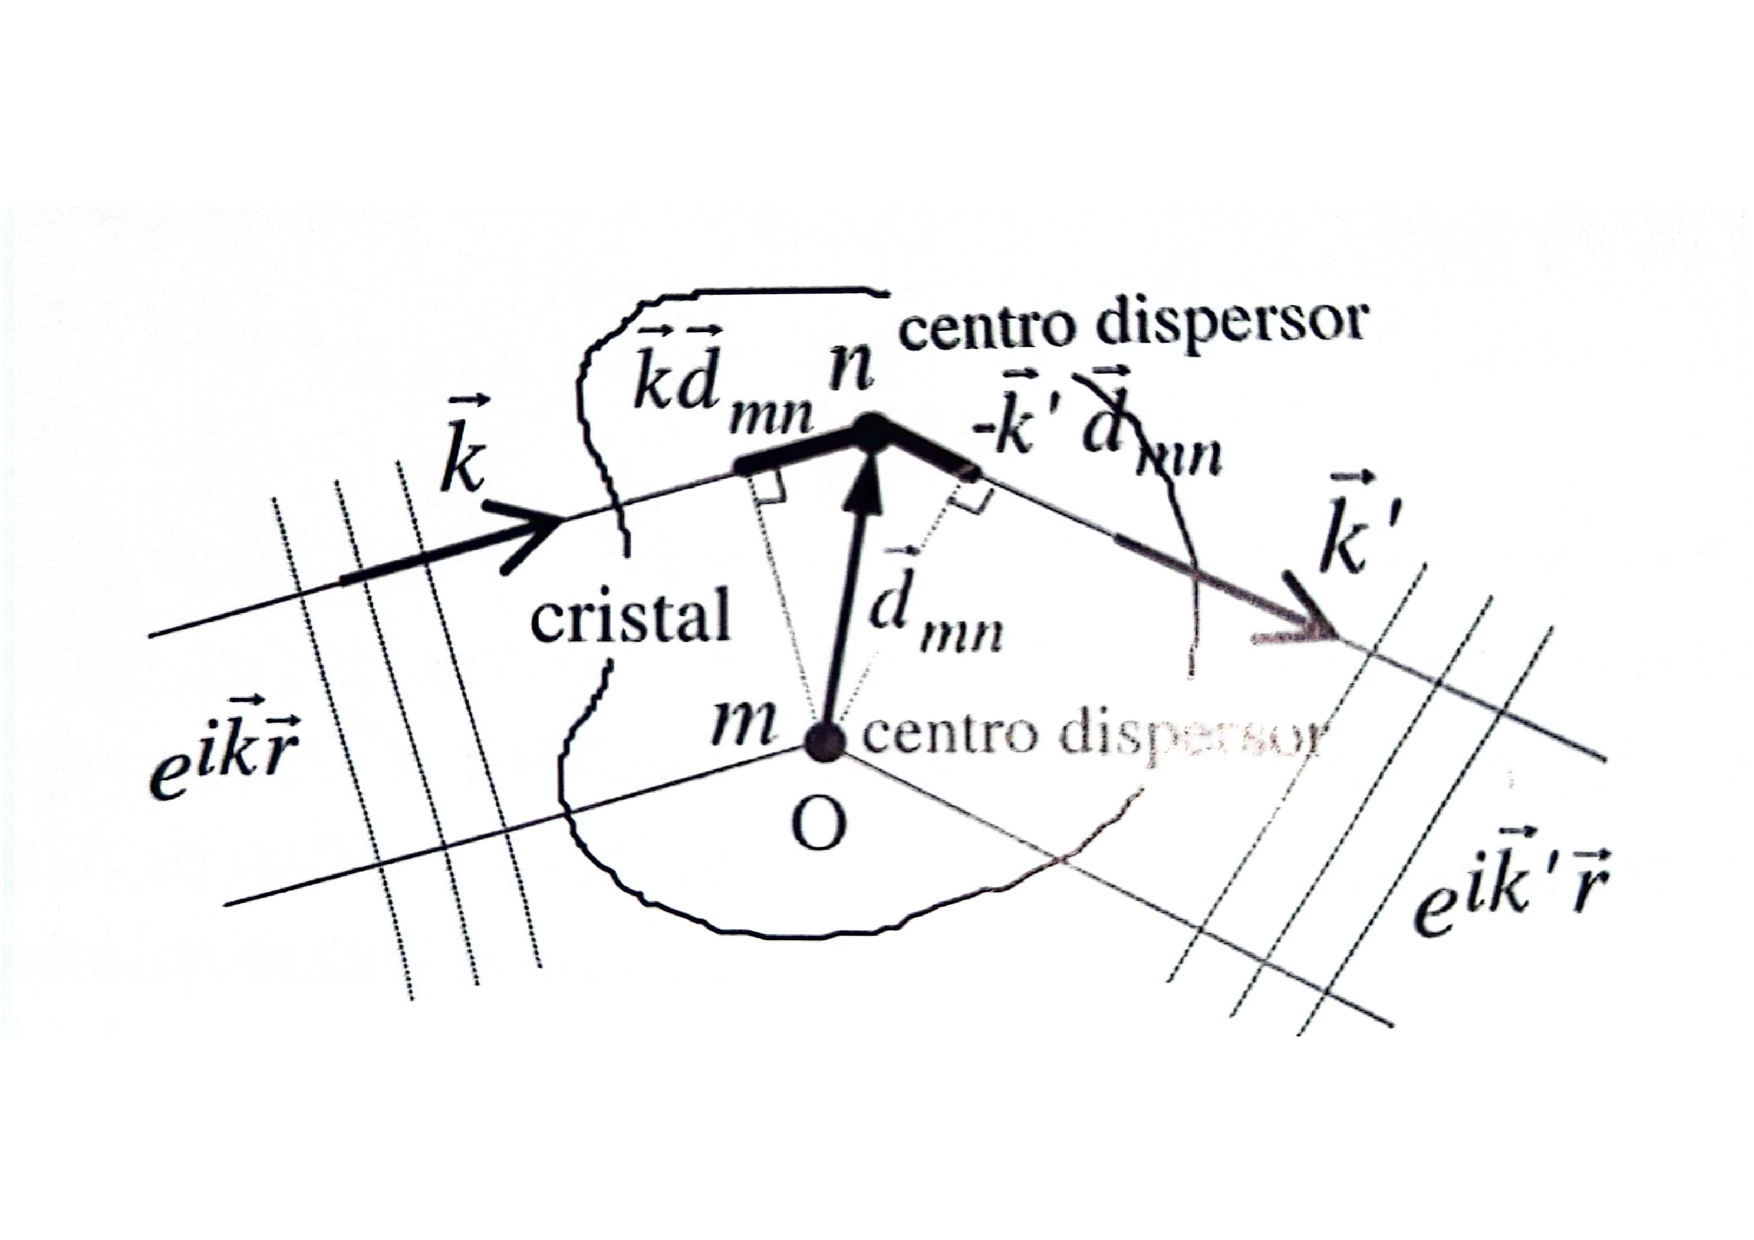
\includegraphics[scale=0.35]{Cuerpo/Ch_02/Fotos_libro 2.pdf}
    \caption{Diferencia de camino recorrido por las ondas dispersadas por dos centros m,n separados $\dn_{mn}$.}
    \label{Fig:02-02}
\end{figure}

Según se indica $\dn_{mn}=\Rn_n+\rn_j$ con lo cualquiera

\begin{equation}
    A_{\text{salida}} \propto  \sum_{n,j} f_j e^{-i (\Rn_n + \rn_j) \cdot \Delta \kn} = \sum_j^{\text{base}} f_j e^{-i \rn_j \cdot \Delta \kn} \sum_{n}^{\text{red}} e^{-i\Rn_n \cdot \Delta \kn} \label{Ec:02-02-02}
\end{equation}
con $\Delta \kn = \kn' - \kn$. A $f_j$ es el llamado \textit{fator de forma atómico}, que da cuenta del distinto \textit{poder dispersor} de los átomos de la base. El máximo de $A_{\text{salida}}$ lo marca el segundo factor que suma a toda la red, pues es una suma del orden de $10^{23}$ términos frente a unos pocos del primero. Este máximo se alcanza con la condición de que

\begin{equation}
    \Delta \kn \cdot \Rn_n = 2 \pi \times \text{entero} \label{Ec:02-02-03}
\end{equation}
para cualquier vector de red $\Rn_n$. La interpretación es que todas las celdas (son las celdas las que están concetadas por vectores de red) deben reemitir en fase para que la suma sea máxima (ver figura \ref{Fig:02-04}).
    
\begin{figure}[h!] \centering
    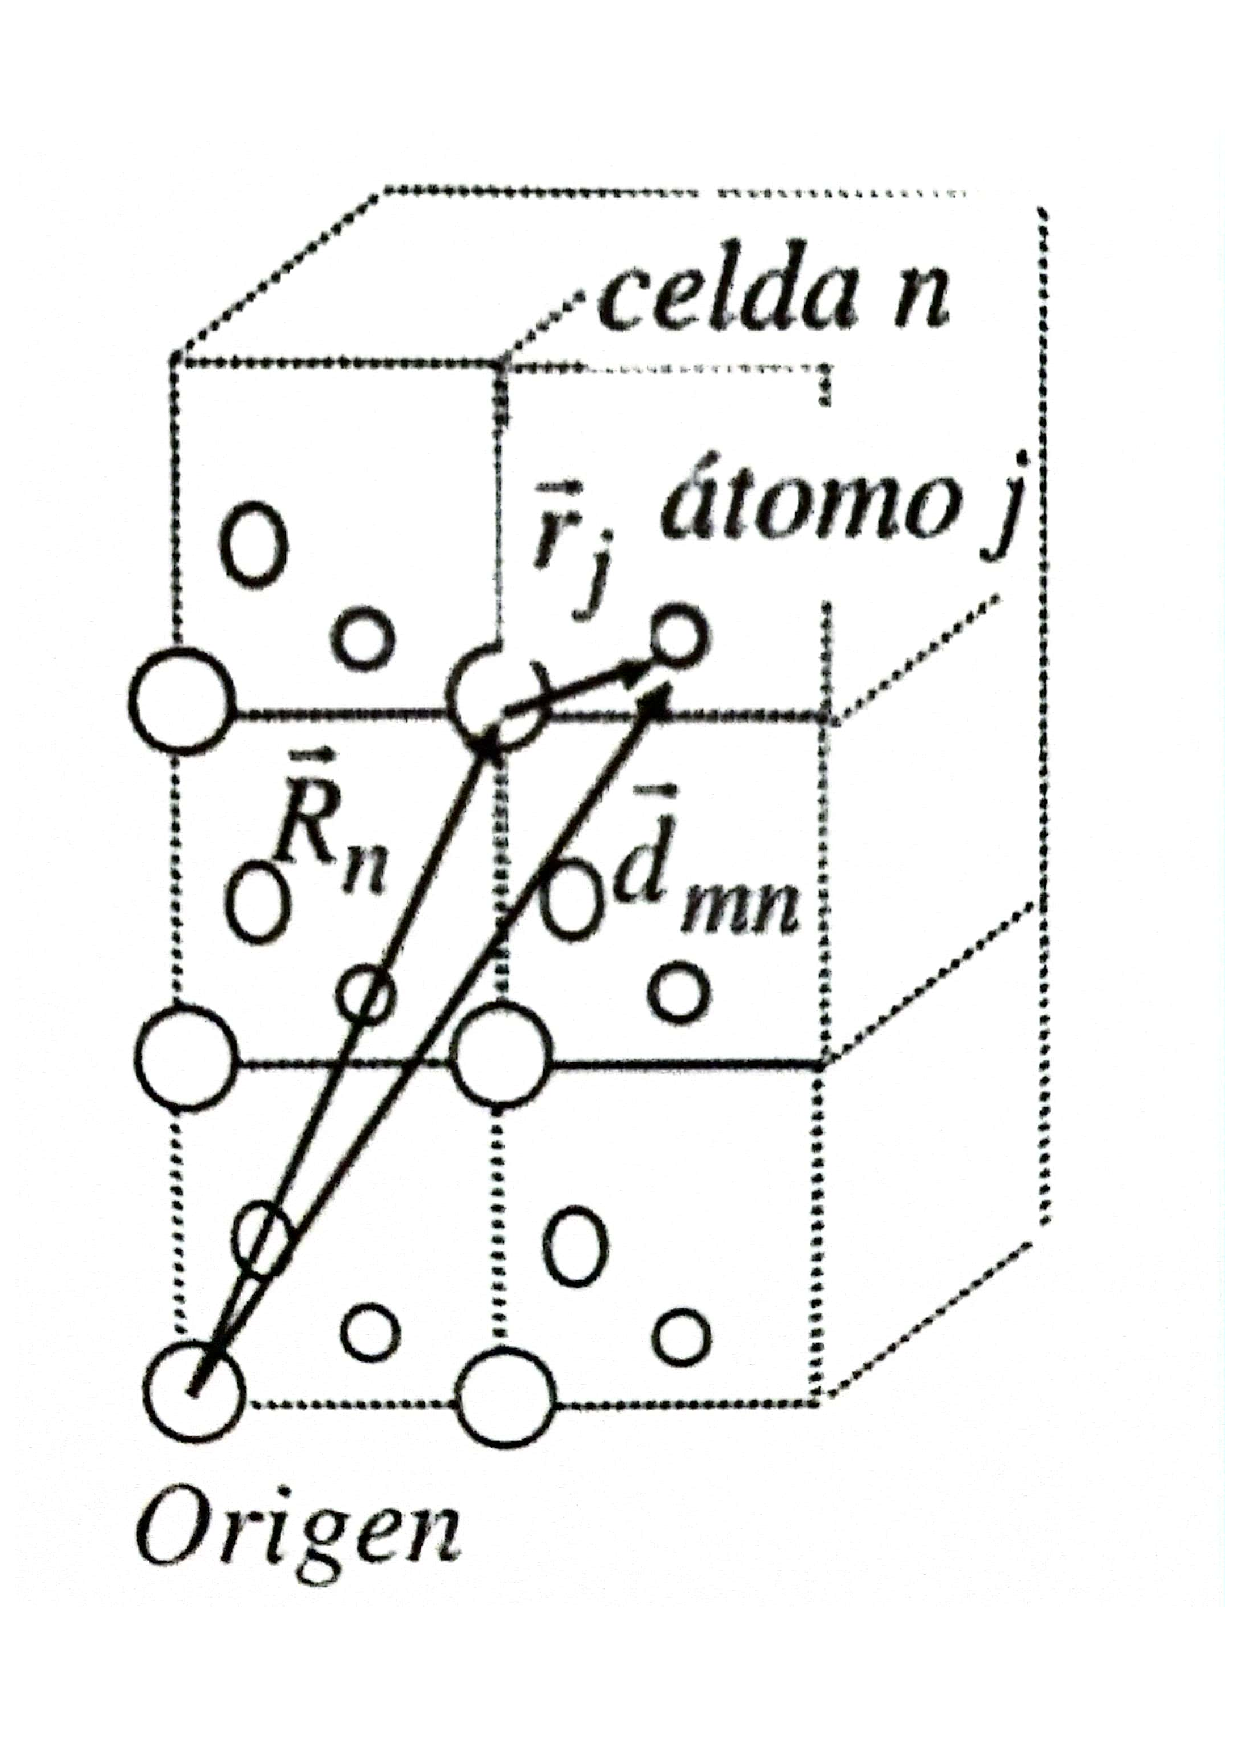
\includegraphics[scale=0.30]{Cuerpo/Ch_02/Fotos_libro 3.pdf}
    \caption{Posición de los centros dispersonres de cada celda $n$ en posición $\Rn_n$.}
    \label{Fig:02-03}
\end{figure}



La condición \ref{Ec:02-02-03} para $\Delta \kn$ es precisamente la definición de red recíproca. Así pues, el resultado básico es que para que haya máximo de difracción (interferencia constructiva) se debe satisfacer 


\begin{equation}
    \Delta \kn = \Gn\label{Ec:02-02-04}
\end{equation}
o bien $\kn'=\kn+\Gn$. Elevando la ecuación \ref{Ec:02-02-04} y teniendo en cuanta que $|\kn|=|\kn'|$ es inmediato ver que esta condición se puede escribir en función del vector de ondas de la radiación incidente y de los vectores de la red recíproca del cristal: $2\kn \cdot \Gn + |\Gn|^2 = 0$. Reemplazando $\Gn$ por $-\Gn$ en esta expresión, la condición de difracción es: 

\begin{equation}
    2 \kn \cdot \Gn = |\Gn|^2 \Longleftrightarrow \kn \cdot \Gn = \frac{1}{2} |\Gn|  \Gn\label{Ec:02-02-05}
\end{equation}
y la dirección en la que se observa el máximo es entonces $\kn'=\kn-\Gn$. 


\begin{figure}[h!] \centering
    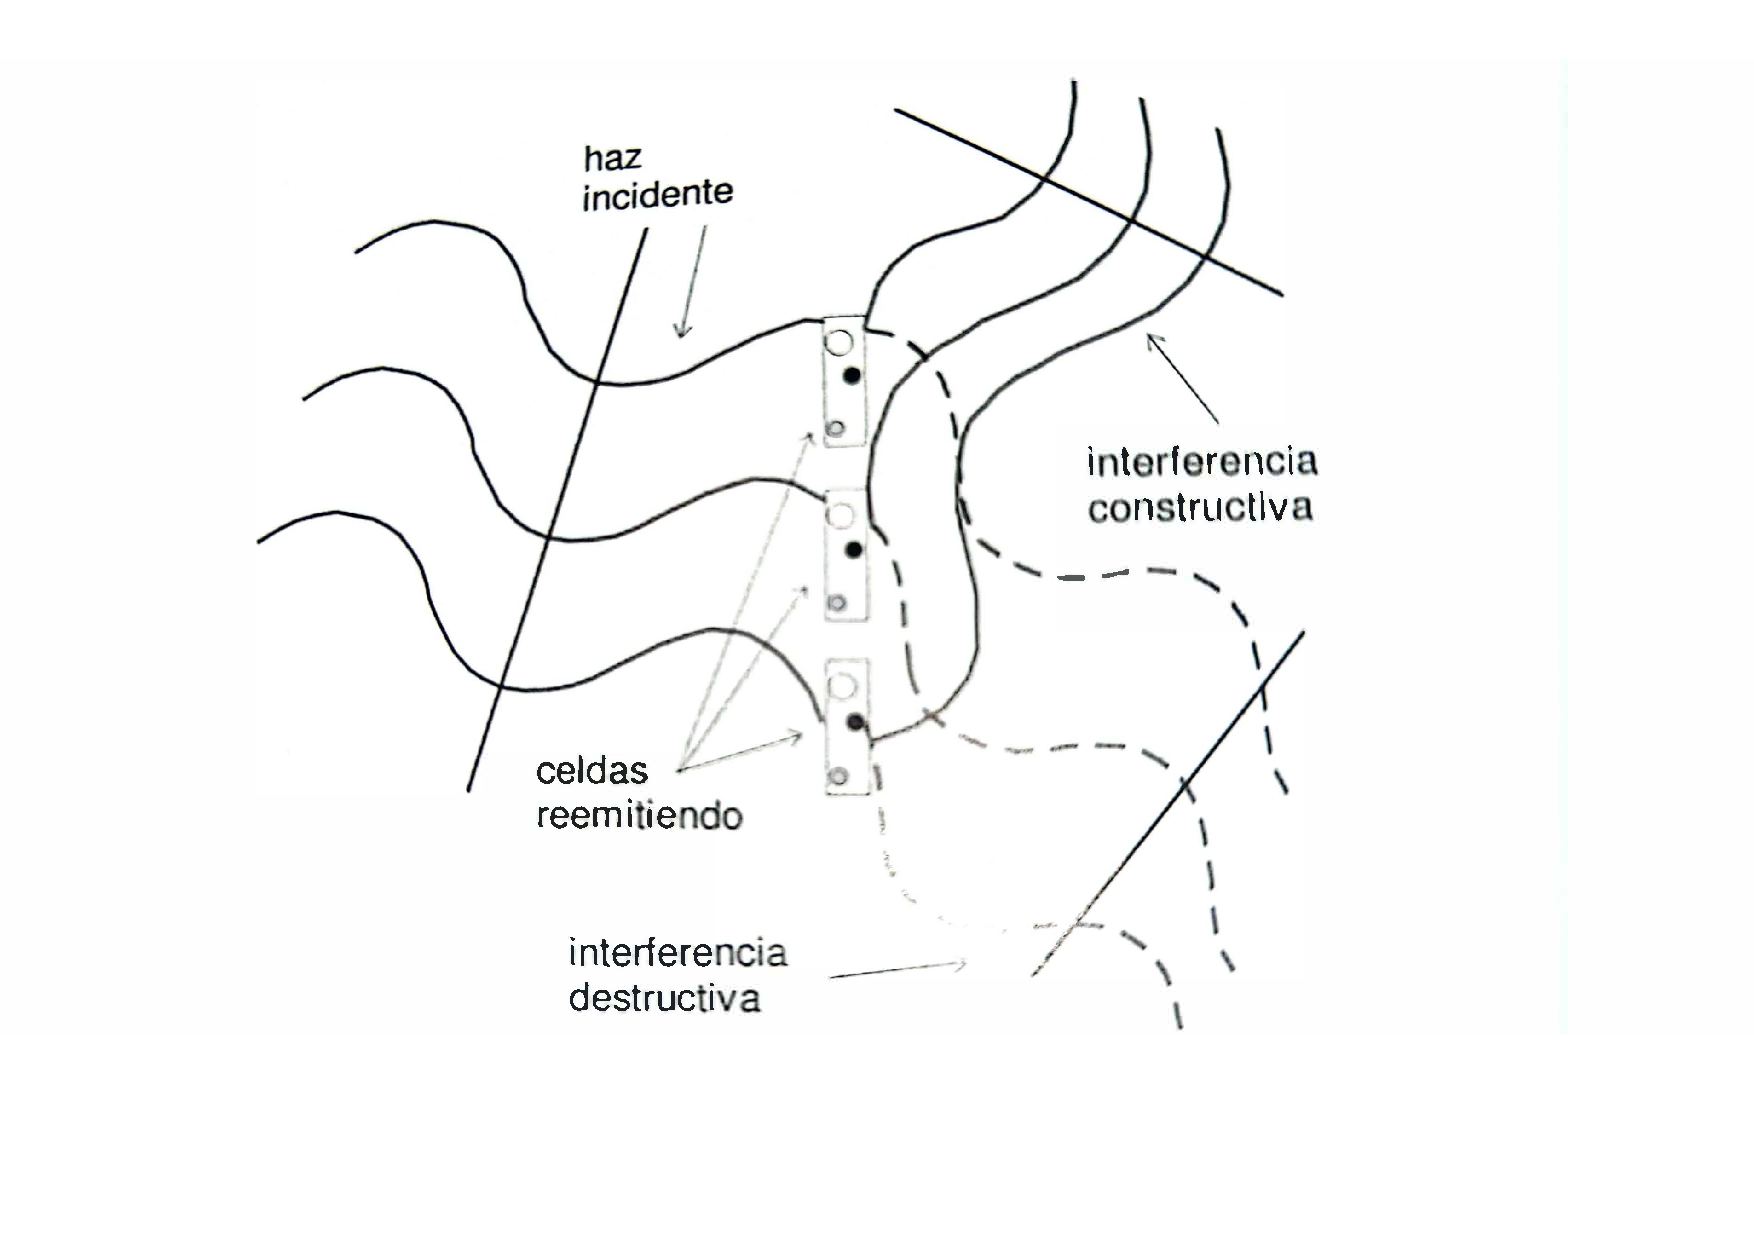
\includegraphics[scale=0.40]{Cuerpo/Ch_02/Fotos_libro 4.pdf}
    \caption{Reemisión de las celdas en fase o no según la dirección considerada}
    \label{Fig:02-04}
\end{figure}

Llamando \textit{plano Bragg} a aquel que es mediatriz a cualquier vector de red de la red recíproca, la interpretación de \ref{Ec:02-02-05} es que se da la condición de difracción para los índices $\kn$ incidentes tales que, con origen en un punto cualquiera de la red recíproca su extremo caiga sobre un plano de Bragg (figura \ref{Fig:02-05}). En particular, lo anterior es válido para la frontera de la \textit{PZB} por estar formada por planos de Bragg. 

\begin{figure}[h!] \centering
    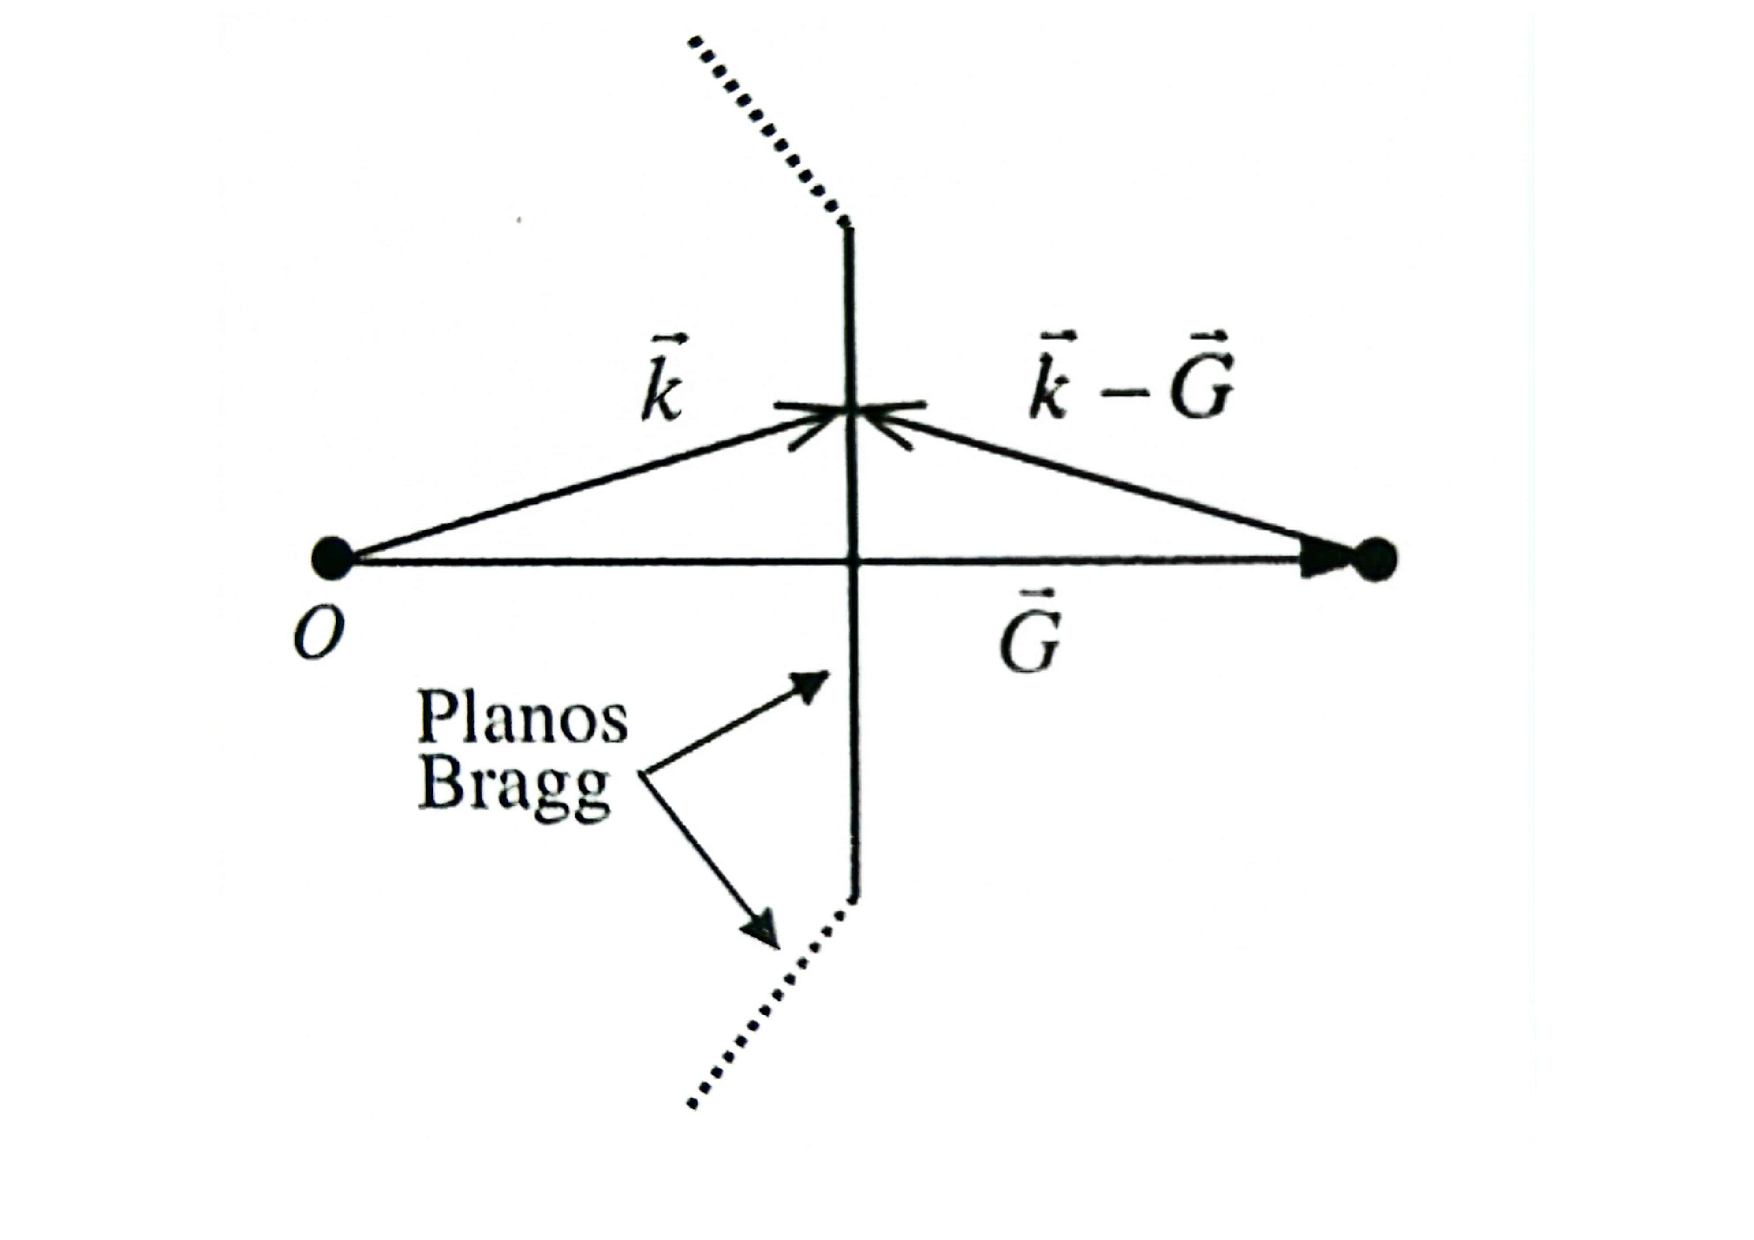
\includegraphics[scale=0.35]{Cuerpo/Ch_02/Fotos_libro 5.pdf}
    \caption{Equivalencia geométrica de la condición de difracción dada por la Ec. \ref{Ec:02-02-05}.}
    \label{Fig:02-05}
\end{figure}

Otra formulación equivalente de la condición de difracción es la llamada \textbf{ley de Bragg} (2013), que admite que la radiación sufre una reflexión especular en los distintos planos reticulares (figura \ref{Fig:02-06}) de modo que sólo si las reflexiones de dos sucesivos planos están en fase se observará máximo de difracción. Es muy fácil de ver que la diferencia de caminos entre planos sucesivos es de $2d\sin \theta$ por lo que esta cantidad deberá ser múltiplo entero de longitudes de onda $\lambda$, es decir,

\begin{equation}
    n \lambda = 2 d \sin (\theta) \label{Ec:02-02-05}
\end{equation}
La equivalencia de la ley de Bragg (ecuación \ref{Ec:02-02-05}) con la formulación más general de las ecuaciones \ref{Ec:02-02-03} y \ref{Ec:02-02-04} se deduce la correspondencia vista entre vectores de la red recíproca y sistemas de planos reticulares. En efecto, el vector $\Gn$ a que hace referencia \ref{Ec:02-02-04} de componentes ($h' k' l'$) no necesariamente primos entre sí, verifica $G=2k\sin \theta$ (figura \ref{Fig:02-07}). Sea ahora $\Gn_0$ el vector de la red recíproca paralelo a $\Gn$ más corto, que debe tener componentes ($hkl$) primas entre sí (por no haber otro más corto), y que verifica $\Gn = n \Gn_0$ (en componentes $h'=nh$, $k'=nk$, $l'=nk$). Como $G_0 = 2\pi/d$ (ecuación \ref{Ec:02-01-05}), al sustituir resulta $n2\pi/d=2k\sin (\theta) \Rightarrow n \lambda = 2 d \sin (\theta)$. 

\begin{figure}[h!] \centering
    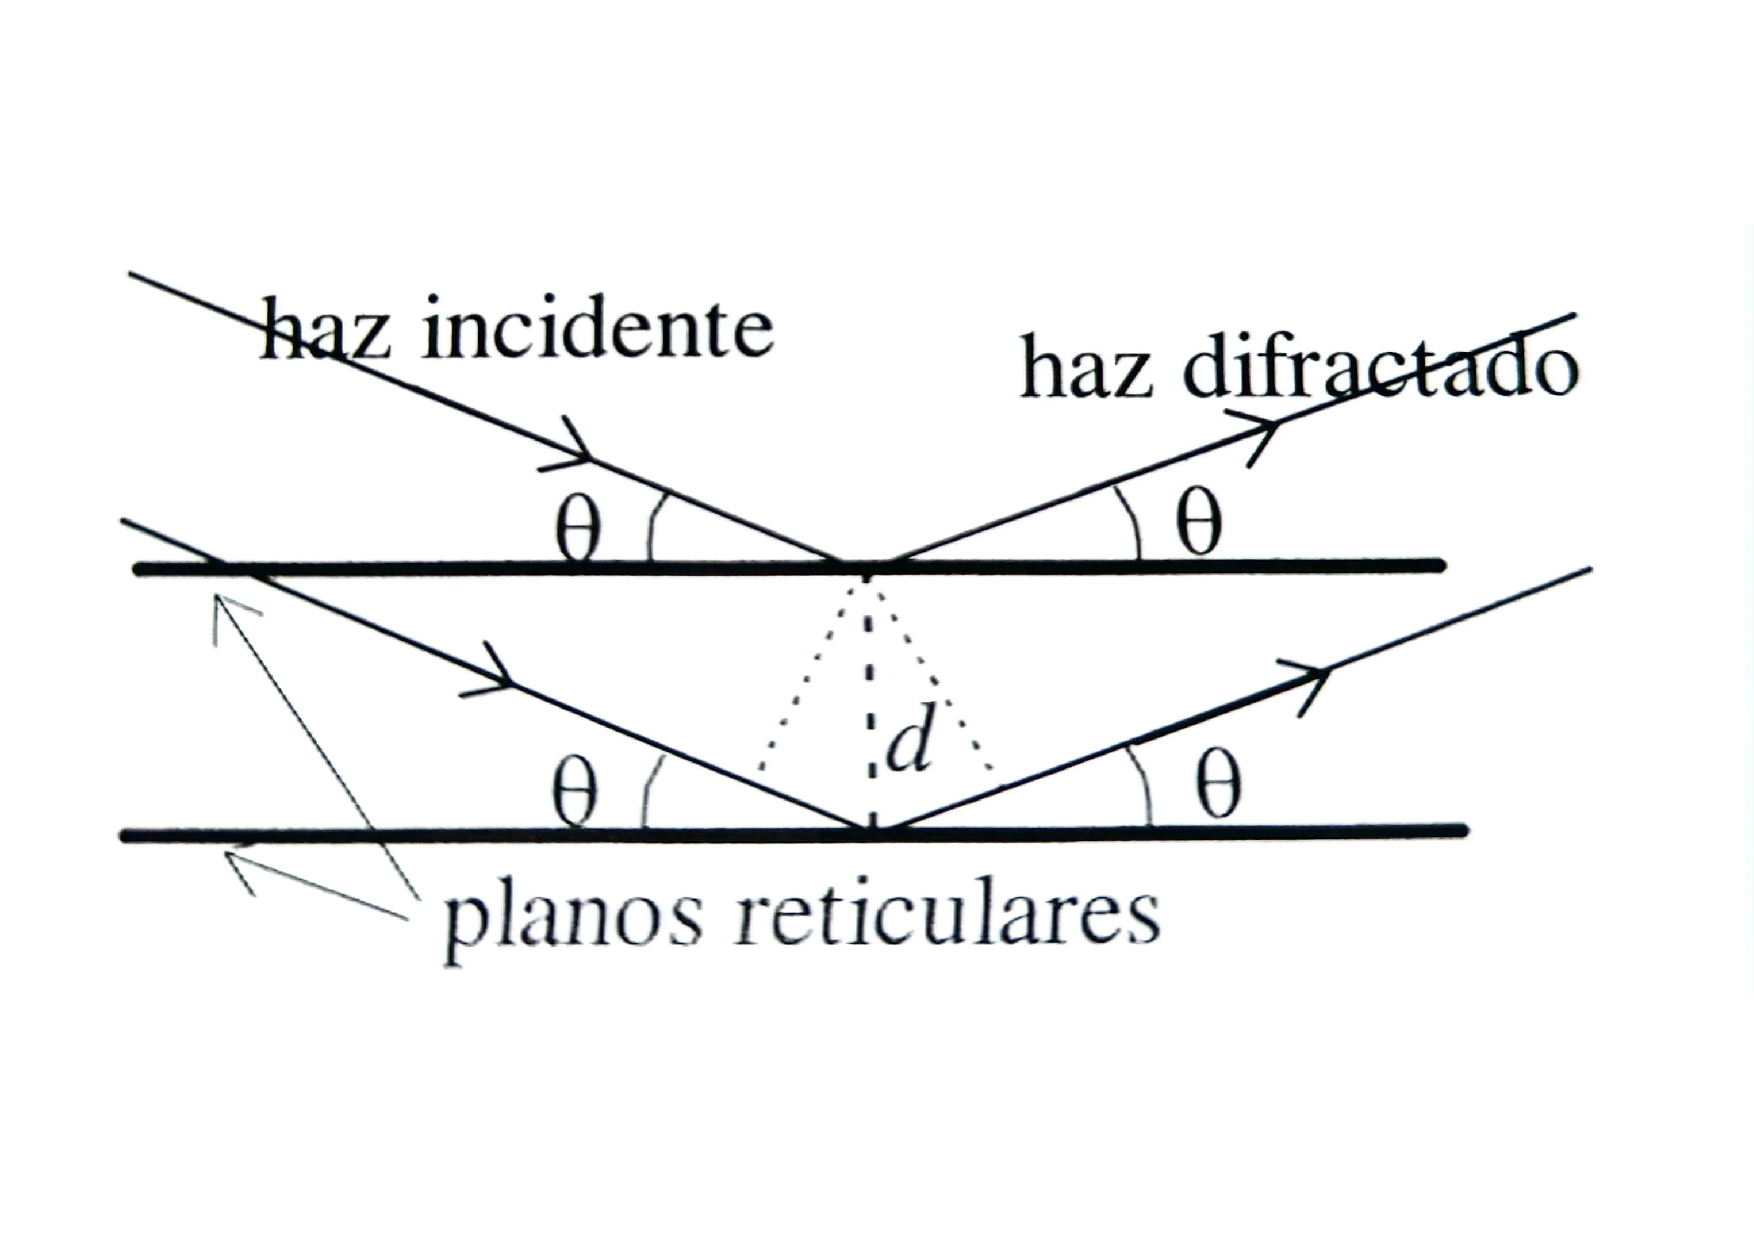
\includegraphics[scale=0.35]{Cuerpo/Ch_02/Fotos_libro 6.pdf}
    \caption{Diferencia de camino recorrido por los haces reflejados especularmente por dos planos reticulares consecutivos.}
    \label{Fig:02-06}
\end{figure}
    
\begin{figure}[h!] \centering
    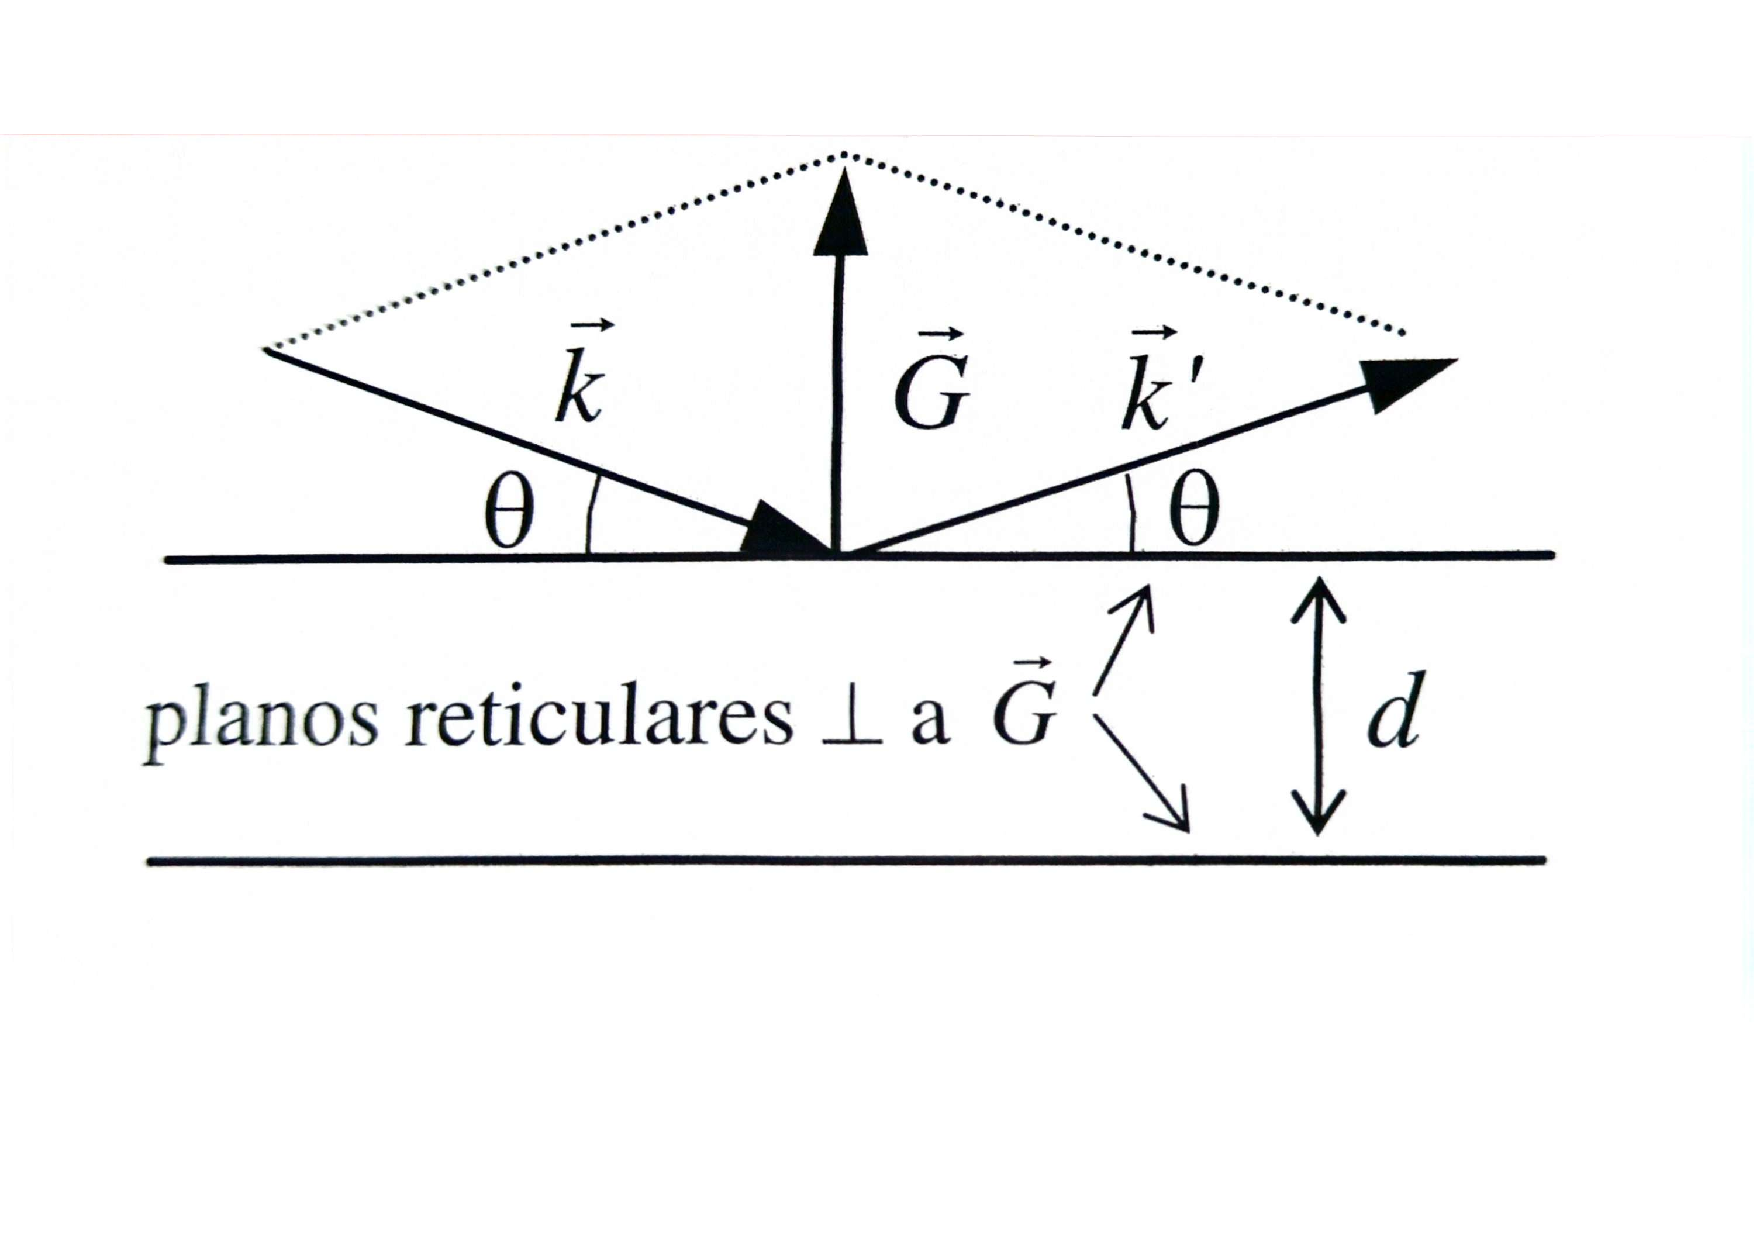
\includegraphics[scale=0.35]{Cuerpo/Ch_02/Fotos_libro 7.pdf}
    \caption{Correspondencia entre vectores de la red recíproca $\Gn$ y sistemas de planos de la red directa.}
    \label{Fig:02-07}
\end{figure}

\section{Factor de estructura}

Se trata de precisar ahora la intensidad de los distintos máximos de difracción. En condición de máximo, la amplitud dispersada (dirección $\hnk'$) es por \ref{Ec:02-02-02} y \ref{Ec:02-02-03}, viene dada por 

\begin{equation}
    A_{\text{salida}} \propto N \sum_j^{\text{base}} f_j e^{-i\rn_j \cdot \Delta \hnk} = N S_{\Gn}
\end{equation}
siendo $N$ el número de celdas. El sumatorio denotado por $S_\Gn$ representa una \textit{suma interferencial dentro de una celda} y se denomina \textit{factor de estructura de la base}.  \\

Para bases poliatómicas puede ocurrir que algunos máximos de difracción permitidos por la red estén prohibidos por la base atómica ($S_\Gn=0$), lo que proporciona una valiosa información sobre su estructura. Por ejemplo, considerando la cúbica \textit{bcc} (monoatómica) como una \textit{sc} con base, están prohibidas las reflexiones \textit{(hkl)} que verifican $h+k+l=$\textit{entero impar}; si se trata de una {\it fcc}  son nulas las reflexiones en que $h,k$ y $l$ tienen \textit{distinta paridad}. Solo quedda por precisar que el factor de forma del átomo genérico $f_j$, a su vez, no es sino una suma interferecnial interna (intraatómica). \

\begin{equation}
    f_j = \int n_j (\rhon) e^{-i \rhon \cdot \Gn} \D^3 \rhon
\end{equation}
siendo $n_j (\rhon)$ la concentración electrónica en el elemento de volumen atómico $\D^3 \rhon$ del átomo $j$, y donde ya se ha supuesto condiciones de máximo de difracción ($\Delta \kn  = \Gn$). El factor de forma atómico, obteniendo de la difracción de rayos x da información de la distribución atómica, observándose diferencias de sólo unos pocos por ciento respecto de los valores teóricas de los átomos libres.

\section{Diagramas de difracción}

La condición de máximo (interferencia constructiva), tal como se expresa por ejemplo en la ley de Bragg, es muy exigente pues para observar un máximo de difracción en cierta dirección [figura \ref{Fig:02-08} (a)] es necesario no sólo que exista un sismtea de planos con la orientación adecuada (con respecto al haz incidente) sino que además tenga el interespaciado preciso dado por la ley de Bragg. Es por eso que para observar máximos experimentalmente se dan más \textit{oportunidades} de cumplimiento girando el cristal según que ejes (\textit{método del cristal giratorio}). Otro médoto consiste en pulverizar la muestra a analizar (\textit{difractograma de polvo}). La presencia de granos cirstalinos orientados al azar hace que los máximos de difracción tengan simetría cilíndrica [figura \ref{Fig:02-08} (b)]. El detector se mueve \textit{barriendo} el ángulo $2\theta$, obteniéndose un diagrama similar al mostrado. 

    
\begin{figure}[h!] \centering
    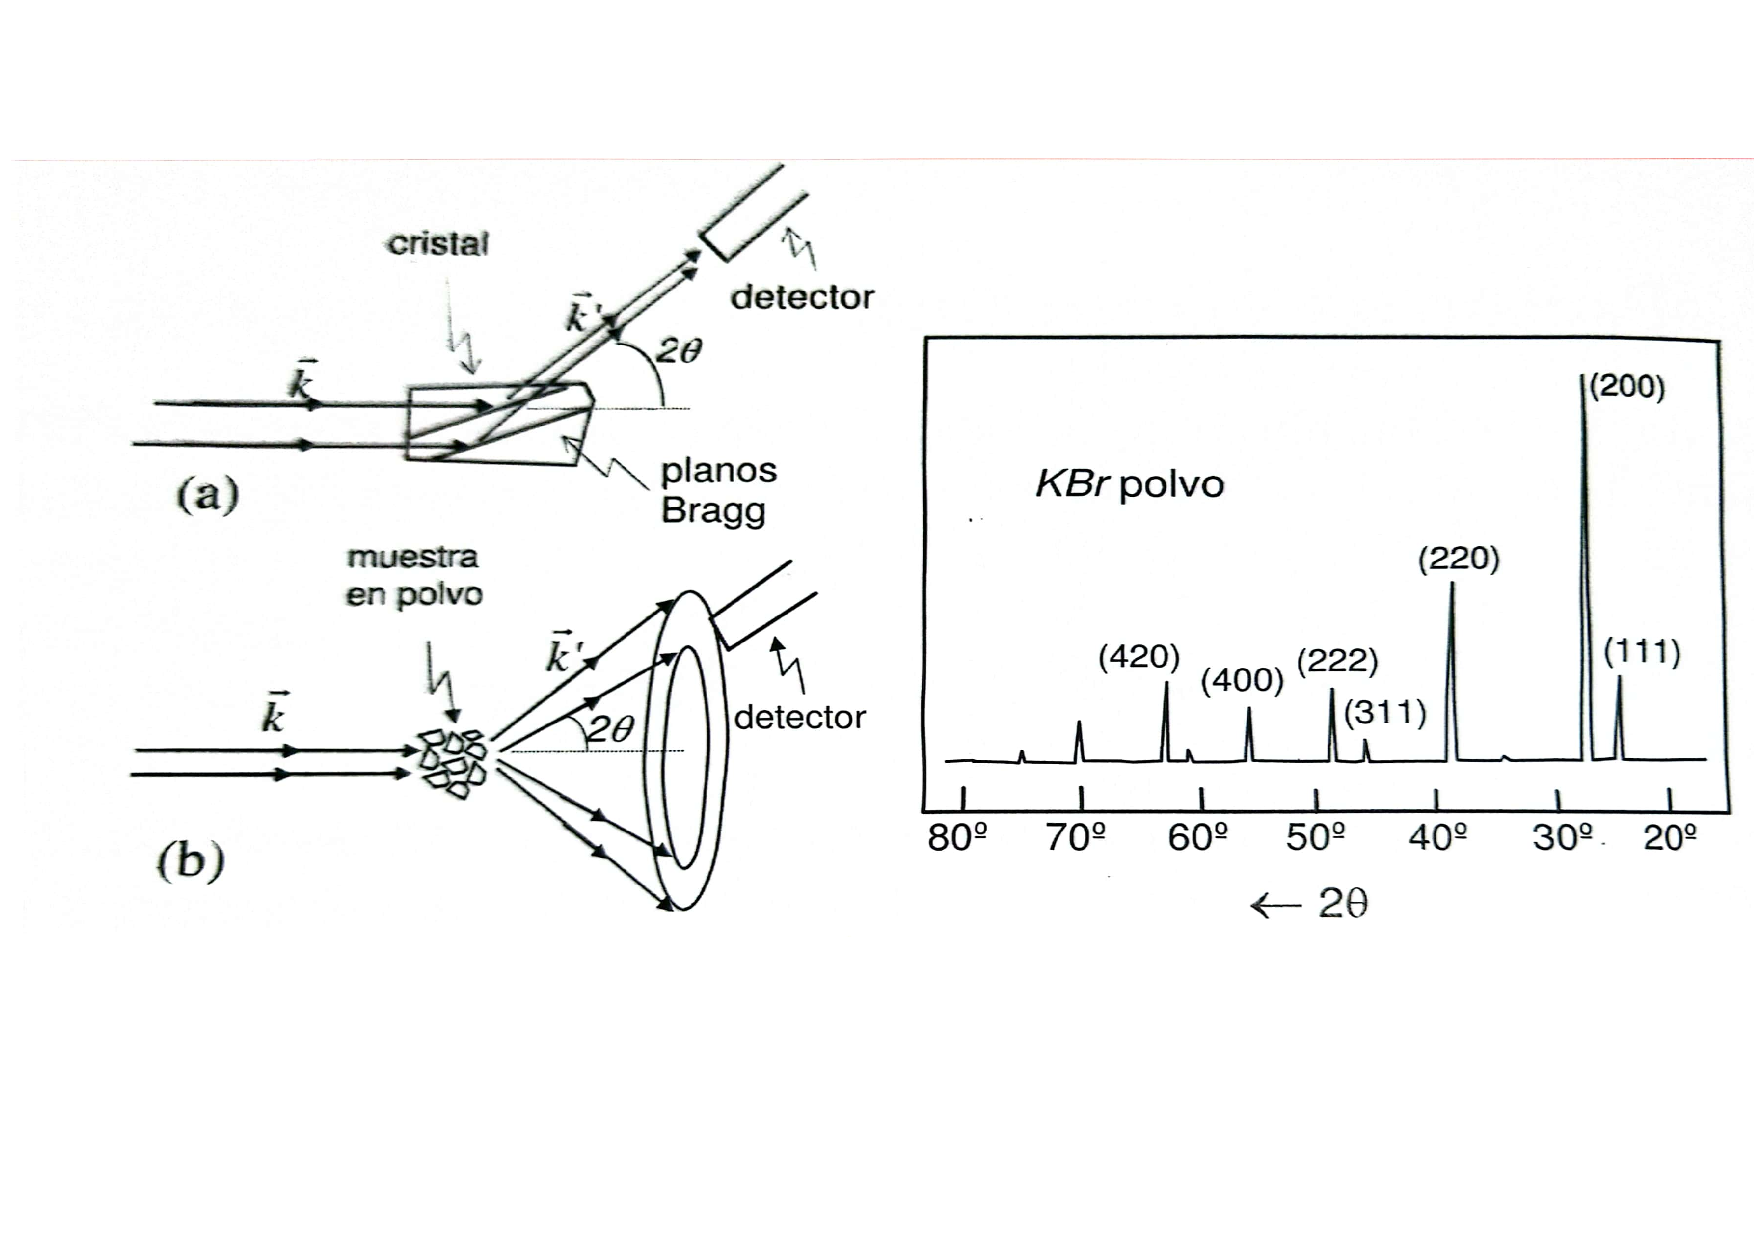
\includegraphics[scale=0.35]{Cuerpo/Ch_02/Fotos_libro 8.pdf}
    \caption{Esquemas de dos métodos de difracción (cristal rotatorio y polvo) y ejemplo de difractrograma que se obtiene.}
    \label{Fig:02-08}
\end{figure}

Tanto la falta de monocormaticidad como de paralelismo del haz incidente contribuyen a ensanchar los máximos. También, los defectos cristalinos afectan a los difractogramas; así la presencia de dislocaciones afecta a la anchura de los máximos de difracción de modo que su análisis se emplea, por ejemplo, para el estudio de defectos de los metales trabajados en frío. La temperatura, que genera vibraciones alrededor de las posiciones de equilibrio, no contribuye sin embargo a ensanchar los picos sino a disminuir su intensidad. Esto se entiende porque a mayor temperatura, en cualquier instante, menos átomso hay en las posiciones regulares (de equilibrio) y, por otro lado, la contribución de los átomos desviados en una determinada dirección, que generaría cambio en el haz difractado, es anulado por los que están desplazados en el sentido opuesto. 
    
\begin{figure}[h!] \centering
    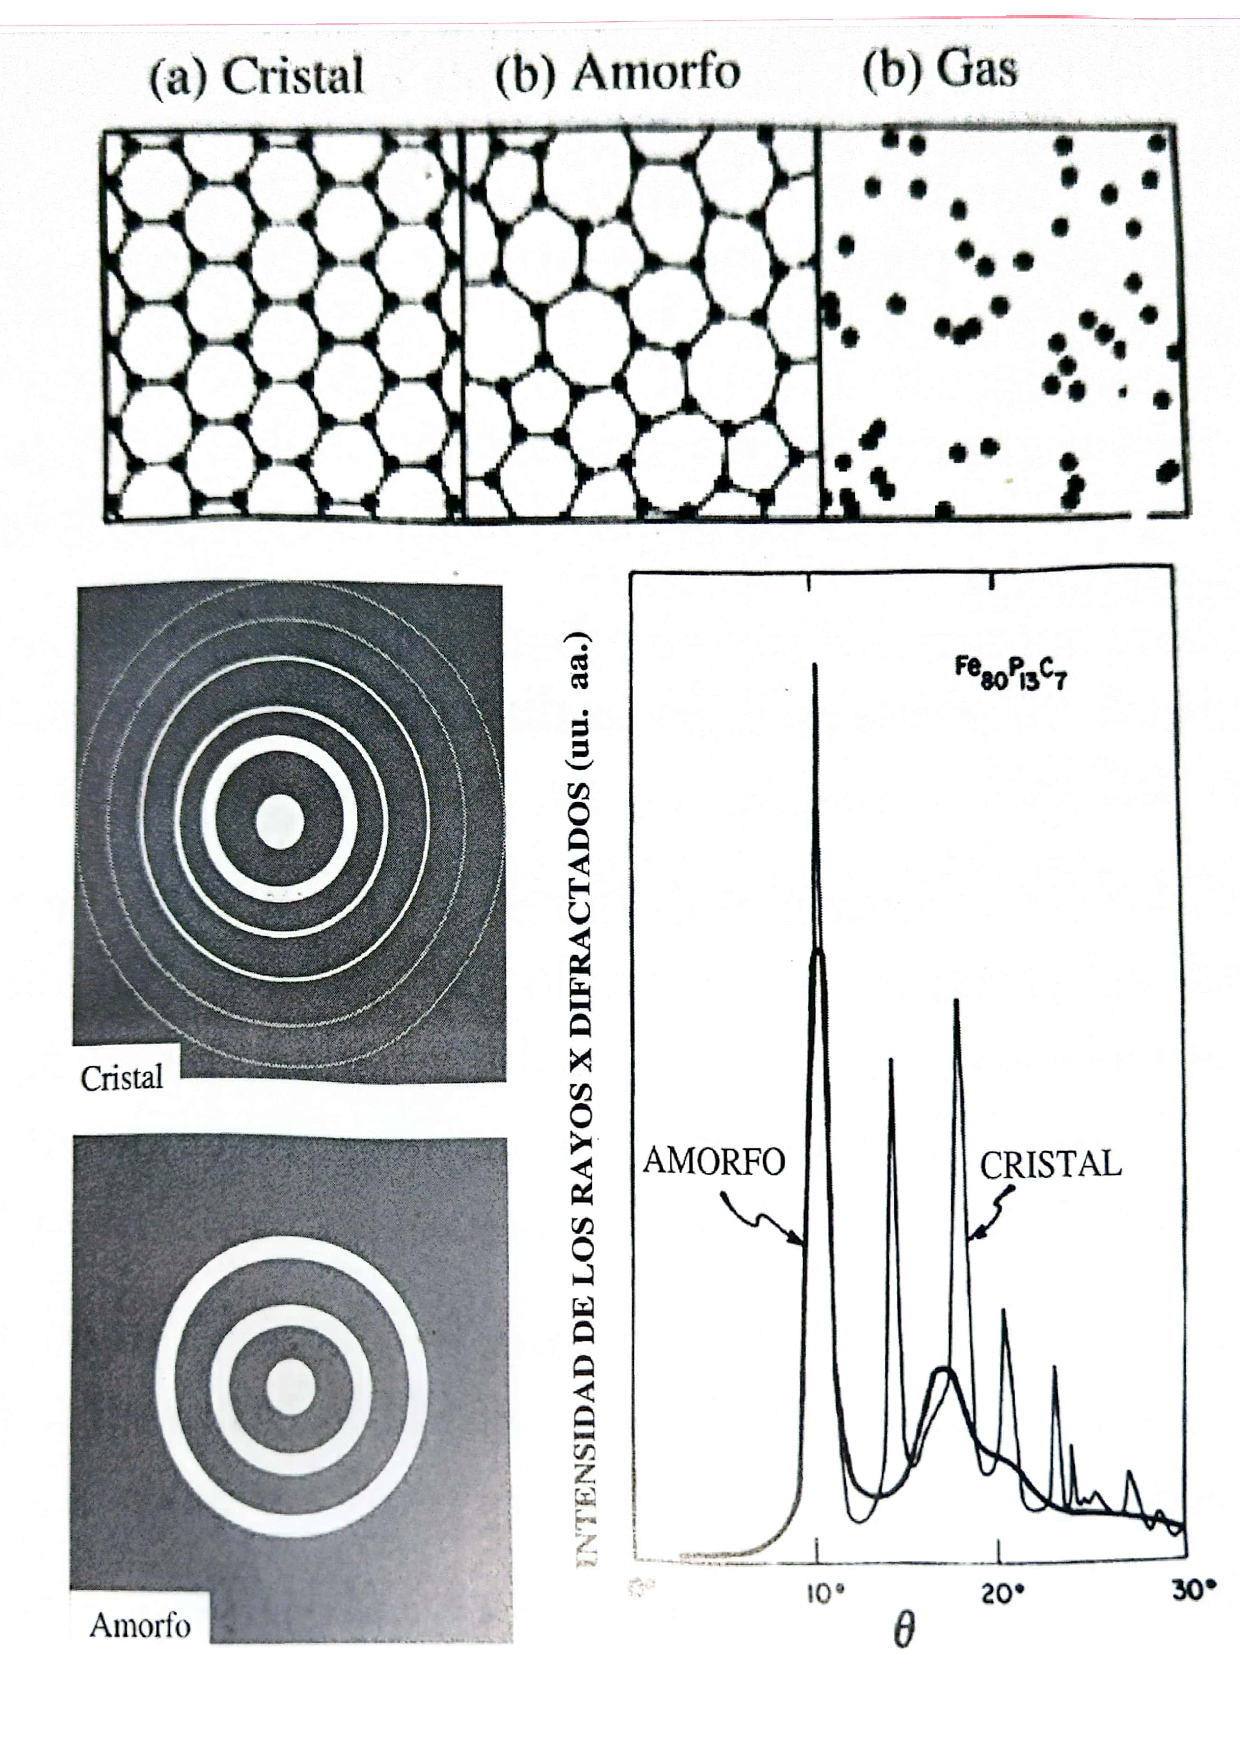
\includegraphics[scale=0.45]{Cuerpo/Ch_02/Fotos_libro 9.pdf}
    \caption{Efecto del desorden atómico en la difracción de rayos x.}
    \label{Fig:02-09}
\end{figure}

Es interesante hacer notar que la existencia de interferencia constructiva de los $N$ átomos de un cristal ($\sim 10^{28} \text{m}^{-23}$) es posible sólo gracias a que éstos están en posiciones regulares, es decir, están \textit{ordenados}. Que el orden está estrechamente asociado a la existencia de máximos de difracción lo muestra la figura \ref{Fig:02-08} donde se ve la correpondencia entre el orden espacial limitado de los materiales que se denominan amorfos con su espectro de difracción. Aquí la existencia de los dos picos de difracción a bajo ángulo está asociada al orden de corto alcance (primeros vecinos) característico de estos materiales.